%%%%%%%%%%%%%%%%%%%%%%%%%%%%%%%%%%%%%%%%%%%%%%%%%%%%%%%%%%%%%%%%%%%%%%%%%%%%%%%%%%%%%%%%%%%%%%%%%%%%%%%%%%5
%%%%%%%%%%%%%%%%%%%%%%%%%%%%%%%%%%%%%%%%%%%%%%%%%%%%%%%%%%%%%%%%%%%%%%%%%%%%%%%%%%%%%%%%%%%%%%%%%%%%%%%%%%%
\section{Other Experiment Techniques}
\subsection{Semi-Inclusive Measurements}
\begin{figure}[!ht]
  \begin{center}
    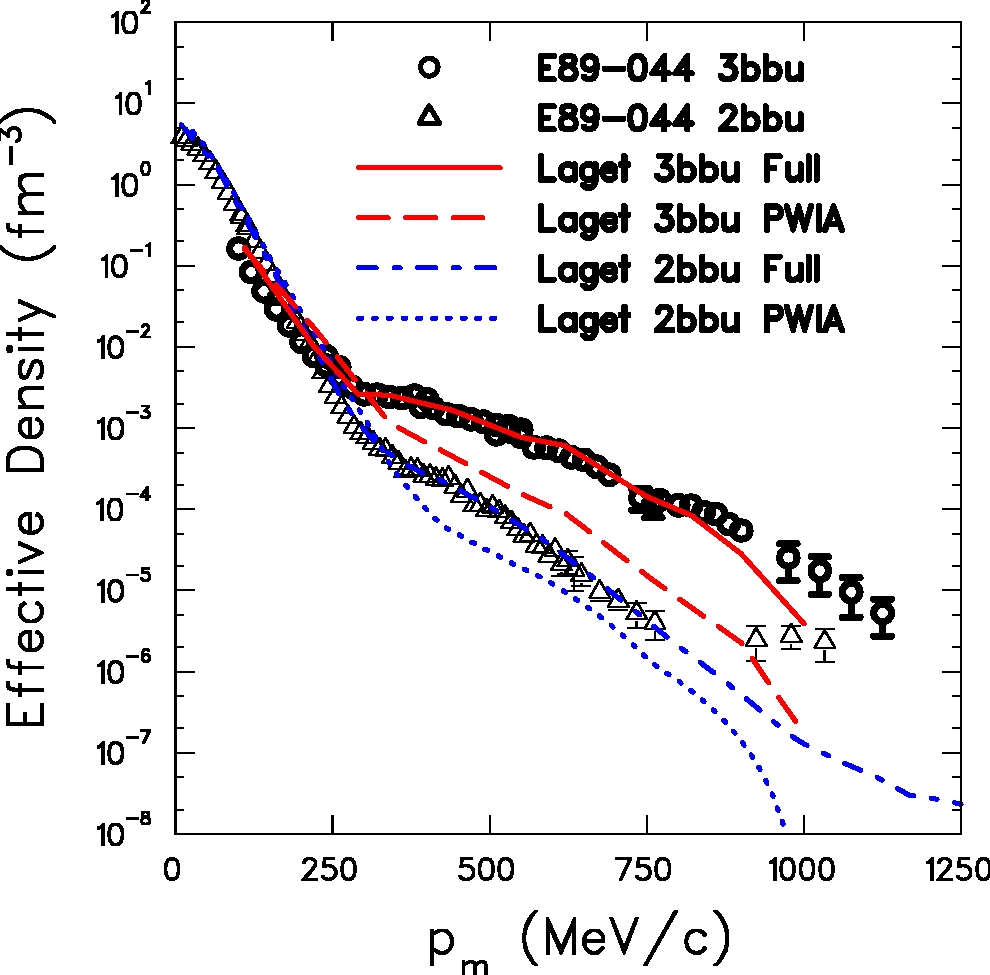
\includegraphics[type=pdf,ext=.pdf,read=.pdf,width=0.60\linewidth]{./figures/physics/10yrSRC_fig3}
    \caption[Proton Effective Momentum distribution in $^{3}He$.]{\footnotesize{Proton Effective Momentum distribution in $^{3}He$~\cite{PhysRevLett.94.082305}, where circles and triangles are experimental data in $^{3}He(e,e'p)pn$ three-body break-up and $^{3}He(e,e'p)d$ two-body break-up, respectively. Lines are theoretical calculations from~\cite{Laget200549}. For the missing momentum above the Fermi momentum (250 MeV), the momentum distribution of three-body break-up is much stronger than the one of two-body break-up, indicating the dominance of SRCs in this region.}}
    \label{10yrSRC_fig3}
  \end{center}
\end{figure} 
Proton-knock-out experiments allow the direct access of the proton's initial momentum distribution through the reconstruction of the nuclear spectral function from the exclusive cross sections. In addition to measuring the scattered electron, one can map out the effect of SRCs to the high momentum tail by detecting the struck proton. Since the correlated nucleon in 2N-SRC is ejected on the opposite direction is not detected, one generally treats the $A(e,e'p)$ reaction as semi-inclusive process. 

To evaluate the deviation of a theoretical calculation of the momentum distribution to the experimental cross section, a normalization factor is introduced in Eq~\eqref{quasi_xs_spectral_function} (for only one proton case)~\cite{Higinbotham:2009hi}:
\begin{equation}
  \frac{d^{6}\sigma}{(dEd\Omega)_{e}(dEd\Omega)_{p}} = K\sigma_{ep}S(E_{0},\mathbf{p_{0}})T_{A}(Q^{2}),
\end{equation}
where $K$ is a kinematic factor and the transparency, $T_{A}$ is the probability that a nucleon will be emitted from the nucleus with other effects, such as FSI. Experiments in Hall-C~\cite{PhysRevLett.80.5072,PhysRevC.66.044613,PhysRevC.72.054602} measured the values of $T_{A}$ for several nuclei which were found to be larger than the predictions in IPSM. Such an enhancement is mainly due to the SRCs effect~\cite{Higinbotham:2009hi}. 

Hall-A experiments ~\cite{PhysRevLett.94.082305,PhysRevLett.94.192302} studied the momentum distribution of $^{3}He$ and observed that the strength greatly increases in the high momentum tail compared with the expected strength including SRCs (Fig.~\ref{10yrSRC_fig3}). This scenario is explained as the combination of SRCs and FSI. 

\subsection{Triple-Coincidence Measurements}
The exclusive cross section measurement of the $A(e,e'pN)$ reaction, or called the triple-coincidence experiment~\cite{PhysRevLett.90.042301,PhysRevLett.99.072501,src_since}, is able to direct probe the scattered electron, the struck nucleon and the spectator nucleon in 2N-SRC. Such an experiment not only can directly conform the production of 2N-SRC, but also can study the types of the nucleon pairs involved in the correlation.  
\begin{figure}[!ht]
  \begin{center}
    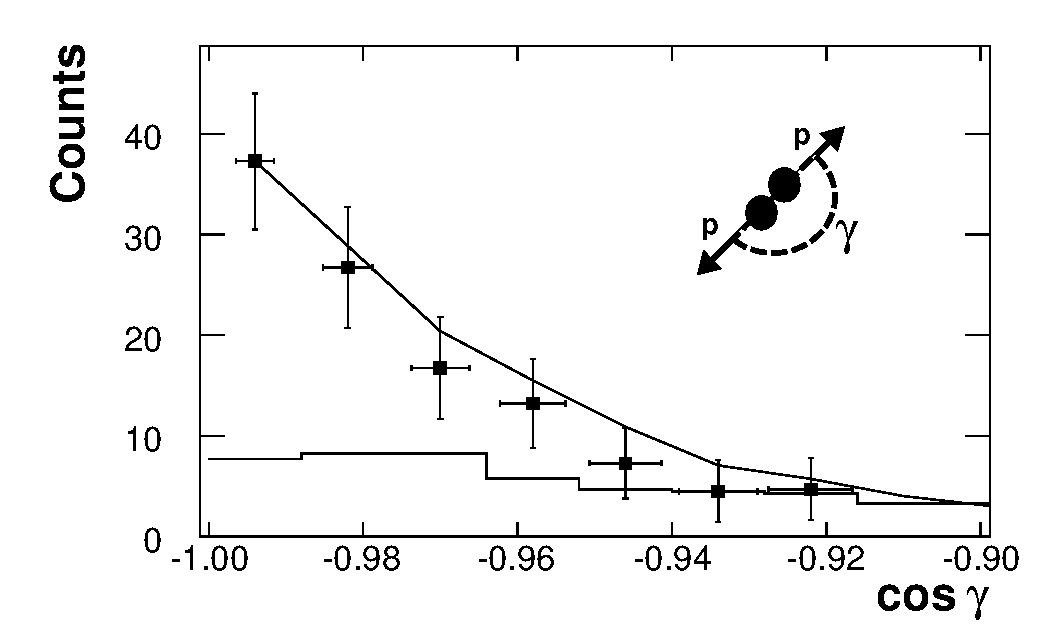
\includegraphics[type=pdf,ext=.pdf,read=.pdf,width=0.60\linewidth]{./figures/physics/10yrSRC_fig5}
    \caption[Angular correlation between nucleons in 2N-SRC]{\footnotesize{Angular correlation between nucleons in 2N-SRC, where the x-axis is the cosine of the opening angle between the struck nucleon and the spectator nucleon in the $^{12}C(e,e'pp)$ reaction~\cite{PhysRevLett.99.072501}.}}
    \label{triple_src_cos}
  \end{center}
\end{figure} 

A recent experiment in Hall-A, E01-015, ~\cite{PhysRevLett.99.072501,src_since}, has performed such a measurement using electron scattering on carbon target. In the $^{12}C(e,e'pp)$ reaction, the experiment studied the angular correlations between the struck proton and the spectator nucleons. Fig.~\ref{triple_src_cos} gives the distribution of the events in $cos\gamma$ when $p_{m}$=500~MeV/c, which clearly peaks near $cos\gamma=-1$. This result proved that the correlated nucleons are ejected back-to-back from the nucleus. The ratio of $pn$ and $pp$ in 2N-SRC can be extracted by using comparing $^{12}C(e,e'pp)$ and $^{12}C(e,e'pn)$. Fig.~\ref{triple_src_np} shows that the ratio of $np/pp$ pairs is around $18\pm 5$, which conforms that the 2N-SRC is dominated by the two-body tensor interaction. 
\begin{figure}[!ht]
  \begin{center}
    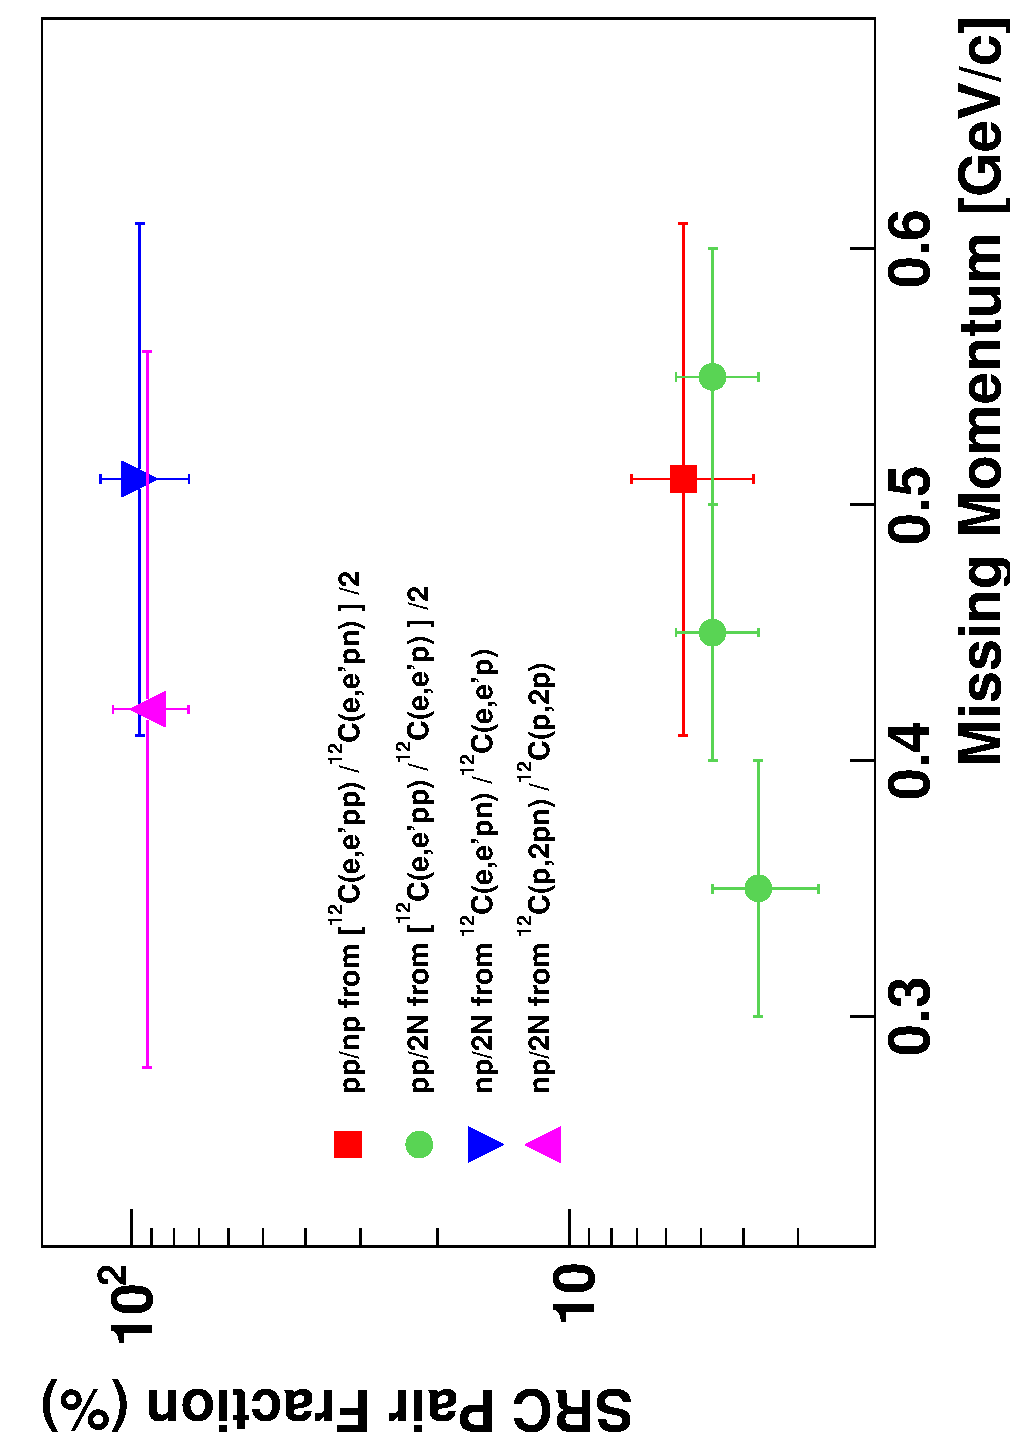
\includegraphics[type=pdf,angle=270,ext=.pdf,read=.pdf,width=0.60\linewidth]{./figures/physics/10yrSRC_fig7}
    \caption[The fraction of $np$ pairs to $pp$ pairs in 2N-SRC]{\footnotesize{The fraction of $np$ pairs to $pp$ pairs in 2N-SRC in carbon from the triple-coincidence experiment in Hall-A~\cite{src_since}.}}
    \label{triple_src_np}
  \end{center}
\end{figure} 